\title{Loom: High performance blockchain }

\author{
        Anatoly Yakovenko \\
        aeyakovenko@gmail.com\\
}
\date{}

\documentclass[12pt]{article}

\usepackage{graphicx}

\begin{document}
\maketitle

\begin{abstract}
A new Proof of History algorithm is proposed for global read consistency which can be used alongside a consensus algorithm to minimize messaging overhead in a Byzantine Fault Tolerant replicated state machine. It achieves performance by creating a single globally agreed upon order of events independent of network consensus. Nodes participating in the network only vote on a binary choice of accepting or rejecting the ordering. Without hardware failures, all the participating nodes are expected to agree with the proposed ordering with minimal communication overhead above the transaction data itself. Any consensus algorithm can be used, such as Proof of Work or Proof of Stake, a simple Proof of Stake consensus algorithm is proposed. To ensure high availability of data, an efficient streaming Proof of Replication is proposed which takes advantage of the time keeping properties provided by Proof of History.  The combination of PoRep and PoH provides a substantial defense against forgery of the ledger in terms of time and storage. The protocol is analyzed on a 1gbps network, and it is shown that throughput is limited by network or ECDSA digests, and with a GPU dedicated to ECDSA digests over \textbf{350k} and up to \textbf{700k} transactions per second with high availability is theoretically possible.

\end{abstract}

\section{Introduction}
This is time for all good men to come to the aid of their party!

%\paragraph{Outline}
%The remainder of this article is organized as follows.
%Section~\ref{previous work} gives account of previous work.
%Our new and exciting results are described in Section~\ref{results}.
%Finally, Section~\ref{conclusions} gives the conclusions.

\section{Design}\label{proof_of_history}

Loom is a Proof of History generator.  It takes a sequence of arbitrary user transactions.  It orders them in the most efficient way to process them, by maximizing memory throughput.  Executes the transactions on the current state that is stored in RAM.  Publishes the transactions and a signature of the state stored in RAM to the replications nodes.  Spools replicate the operations on their copies of the state, and publish their computed hash as confirmations via consensus algorithm.

\begin{figure}
  \begin{center}
    \centering
    \includegraphics[width=0.9\textwidth]{figures/fig_0.5.png}
    \caption[Fig 1]{Transaction flow throught the network.\label{fig_1}}
  \end{center}
  \end{figure}

In the figure above, messages are sent by users into the Loom node, which orders them and broadcasts the order and the resulted computed state to the replicator nodes called Spools.  Spools then send a confirmation message of the computed state hash to the Loom.

Looms are elected by the network via its configured consensus algorithm, such as Proof of Stake or Proof of Work.  More on elections here.

Proof of History sequence guarantees global read consistency for the network that would require an attacker an investment of time to reverse.  A Proof of Stake algorithm is proposed for electing Looms and posting confirmations of the order.  A fast Proof of Replication is proposed for ledger and state availability, and as a defense against forgery attacks.
\section{Design}

\section{Proof of History}\label{proof_of_history}

Proof of History provides a way to cryptographically verify passage of time between two events. It uses a cryptographically secure function whose output cannot be predicted from the input, and must be completely executed to generate the output. The function is run in a sequence, it’s previous output as the current input, periodically recording the current output, and how many times it’s been called. The output can then be recomputed and verified by external computers in parallel by checking each period in parallel on a separate core. Data can be timestamped into this sequence by recording the data and the index it was mixed into the sequence. The timestamp then guarantees that the data was created sometime before this hash was generated in the sequence. Multiple generators can synchronize amongst each other by mixing their state into each others sequences. \\

\subsection{Description}

With a cryptographic function, like a cryptographic hash (sha256, md5,
sha-1), whose output cannot be predicted without running the function,
run the function from some random starting value and take its output
and pass it as the input into the same function again. And record the
number of times the function has been called and the output at each
call. \\\\
\noindent For example: \\\\\noindent
\texttt{
  sha256(\char`\"any random starting value\char`\") $\rightarrow$
  hash1, (n\_count~$=~1$) \\
  sha256(hash1) $\rightarrow$ hash2, (n\_count~$=~2$)\\
  sha256(hash2) $\rightarrow$ hash3, (n\_count~$=~3$)\\
}

\noindent Where \texttt{hashN} represents the actual hash output. \\

Instead of publishing every hash on every index, only a subset of
these hashes could be published at an interval.\\

\noindent For example:\\\\\noindent
\texttt{
 sha256(\char`\"any starting value\char`\") $\rightarrow$ hash1, (n\_count~$=1$)\\
\ldots\\
sha256(hash199) $\rightarrow$ hash200, (n\_count~$=200$)\\
\ldots\\
sha256(hash299) $\rightarrow$ hash300, (n\_count~$=300$)\\
}

This set of events can only be computed in sequence by a single computer thread, because there is no way to predict what the hash value at index $300$ is going to be without actually running the algorithm from the starting value $300$ times.

\begin{figure}
  \begin{center}
    \centering
    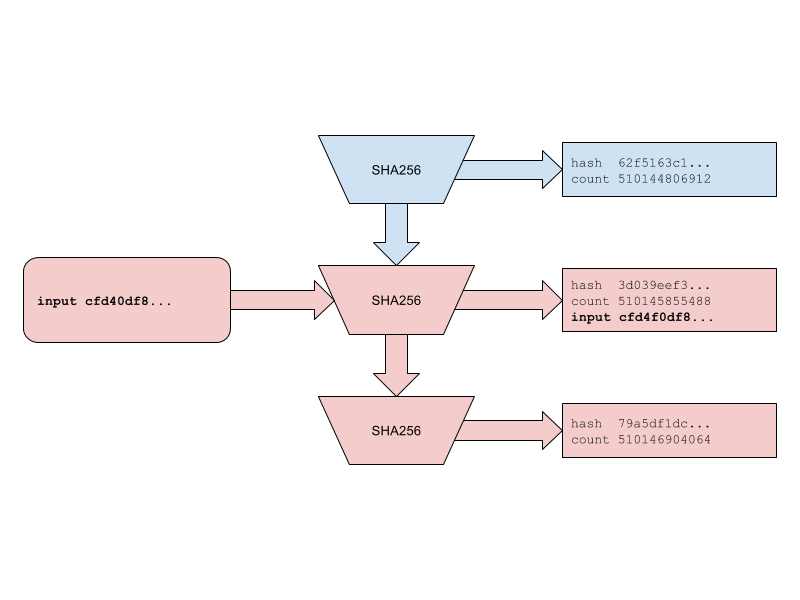
\includegraphics[width=0.6\textwidth]{figures/fig_1.png}
    \caption[Fig 1]{Figure description \label{fig_1}}
  \end{center}
  \end{figure}
%A much longer \LaTeXe{} example was written by Gil~\cite{Gil:02}.
In the example in Figure 1, hash \texttt{62f51643c1} was produced on
count $510144806912$ and hash \texttt{c43d862d88} was produced on
count $510146904064$. Real time passed between count $510144806912$
and count $510146904064$.

\subsection{Timestamp for Events}

This sequence of hashes can also be used to record that some piece of data was created before a particular hash index was generated.  Using a `combine` function to combine the piece of data with the current hash at the current index. The `data` can simply be a cryptographically unique hash of arbitrary event data. The combine function can be a simple append of data, or any operation that is collision resistant.\\

Arithmetic operations like addition, multiplication etc... wouldn’t work because an attacker could have precomputed a separate sequence in parallel, and could join the two by inserting a piece of data that would add up to the starting value of the parallel sequence. Append would force the attacker to try to create a collision between a hash, and the data they are trying to append.\\


\noindent For example:\\\\\noindent
\texttt{
sha256(\char`\"any starting value\char`\") $\rightarrow$ hash1,
(n\_count $=~1$)1\\
\ldots\\
sha256(hash199) $\rightarrow$ hash200, (n\_count $=~200$)\\
\ldots\\
sha256(hash299) $\rightarrow$ hash300, (n\_count $=~300$)\\
}

\noindent Some external event occurs, like a photograph was taken, or
any arbitrary digital data was created:\\\\\noindent
\texttt{
  sha256(hash334) $\rightarrow$ hash335, (n\_count $=~335$), photograph\_sha256\\
  sha256(append(hash335, photograph\_sha256) $\rightarrow$ hash336,
  (n\_count $=~336$)\\
  \ldots\\
  sha256(hash399) $\rightarrow$ hash400, (n\_count $=~400$)\\
}

\texttt{Hash336} is computed from the appended binary data of
\texttt{hash335} and the \texttt{sha256} of the photograph. The index,
and the \texttt{sha256} of the photograph are recorded as part of the
sequence output. So anyone verifying this sequence can then recreate
this change to the sequence. The verifying can still be done in
parallel:\\\\\noindent
\texttt{
  sha256(hash299) $\rightarrow$ hash300, (n\_count $=~300$)\\
  sha256(hash334) $\rightarrow$ hash335, (n\_count $=~335$), photograph\_sha256\\
}\\\noindent
And\\\\\noindent
\texttt{
  sha256(append(hash335, photograph\_sha256) $\rightarrow$ hash336,
  (n\_count $=~336$)\\
  sha256(hash399) $\rightarrow$ hash400, (n\_count $=~400$)\\
}

Because the initial process is still sequential, we can then tell that things entered into the sequence must have occurred sometime before the future hashed value was computed.\\\\\noindent
\texttt{
sha256(hash334) $\rightarrow$ hash335, (n\_count $=~335$), photograph1\_sha256\\
sha256(append(hash335, photograph\_sha256) $\rightarrow$ hash336,
(n\_count $=~336$)\\
\ldots\\
sha256(hash599) $\rightarrow$ hash600, (n\_count $=~600$), photograph2\_sha256
sha256(append(hash600, photograph2\_sha256) $\rightarrow$ hash601,
(n\_count $=~601$)\\
}

So \texttt{photograph2} was created before \texttt{hash601}, and
\texttt{photograph1} was created before \texttt{hash336}. Inserting this extra data into the sequence of hashes results in an unpredictable change to all subsequent values in the sequence. So it would be impossible to precompute any future sequences based on prior knowledge of what data will be mixed into the sequence.\\

The sequence only needs to mix and publish a hash of the event data into the event sequence. The mapping of the hash to event data can be stored outside of the sequence, and the event data can contain other metadata within itself, such as real time stamps and connection IPs.\\

\begin{figure}
  \begin{center}
    \centering
    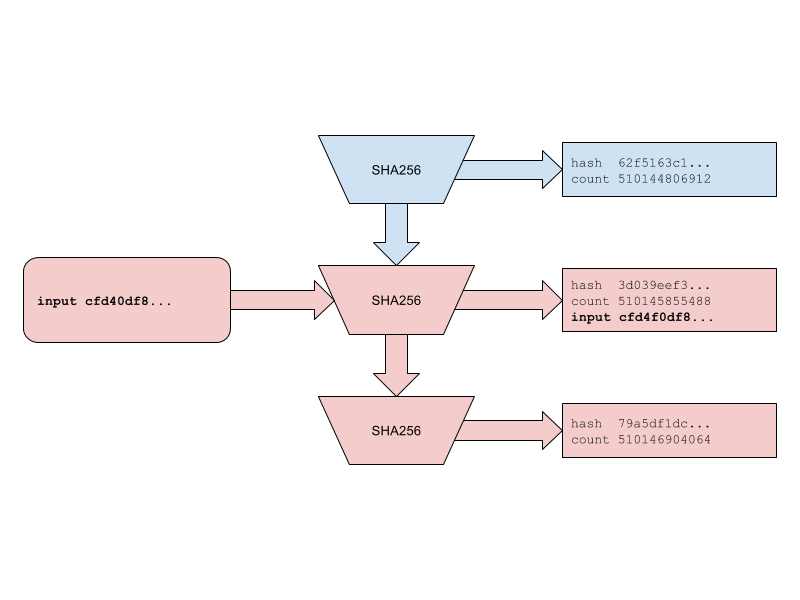
\includegraphics[width=0.9\textwidth]{figures/fig_2.png}
    \caption[Fig 2]{Figure description \label{fig_2}}
  \end{center}
  \end{figure}

  In the example in Figure 2, input \texttt{cfd40df8\ldots} was inserted into the Proof of History sequence. The count at which it was inserted is $510145855488$ and the state at which it was inserted it is \texttt{3d039eef3}.\\

Every node observing this sequence can determine the order at which all events have been inserted. Generating a reverse order would require an attacker to start the malicious sequence after the second event. This delay would allow any non malicious peer to peer nodes to communicate about the original order.\\

\subsection{Timestamp for Events}
\subsection{Verification}
The sequence can be verified as correct in a multi core computer in less time than it took to generated it 

\noindent For example: \\\\\noindent
\texttt{
Core1:
sha256(\char`\"any random starting value\char`\") $\rightarrow$ hash1, 1\\
...\\
sha256(hash199) $\rightarrow$ hash200, 200\\

Core2:\\
sha256(hash199) $\rightarrow$ hash200, 200\\
...\\
sha256(hash299) $\rightarrow$ hash300, 300\\
}

So given some number of cores, like a modern GPU with 4000 cores, the verifier can split up the sequence of hashes and their indexes into 4000 slices, and in parallel make sure that each slice is correct from the starting hash to the last hash in the slice.  So if the expected time to produce the sequence is going to be 

<number of hashes>/<hashes per second for 1 core>

the expected time to verify that the sequence is correct is going to be 

<number of hashes>/(<hashes per second per core> * <number of cores available to verify>)

\begin{figure}
  \begin{center}
    \centering
    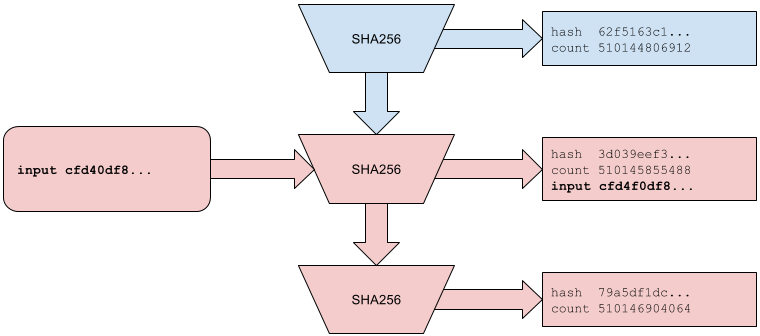
\includegraphics[width=0.9\textwidth]{figures/fig_3.png}
    \caption[Figure 3]{Verification using multiple cores\label{fig_3}}
  \end{center}
  \end{figure}

In the example in Figure 3, each core is able to verify each slice of the sequence in parallel.  Since all input strings are recorded into the output, with the counter and state that they are appended to, the verifiers can replicate each slice in parallel.
\subsection{Verification}


\section{Results}\label{results}
In this section we describe the results.

\section{Conclusions}\label{conclusions}
We worked hard, and achieved very little.

\bibliographystyle{abbrv}
\bibliography{simple}

\end{document}
This is never printed
